  \section{Network}
  \begin{frame}
    \frametitle{Aims}
      \begin{itemize}
        \item Interface transport layer,
	\item Host addressing,
        \item End-to-end packet transmission (data link? Connectionless? Switch? Router?),
        \item Routing, load balancing
      \end{itemize}
  \end{frame}
  \begin{frame}
    \frametitle{Concepts}
      \begin{itemize}
        \item IP addressing fundamentals,
        \item Classfull IP addressing,
        \item Subnet and VLSM (Variable length subnet masks),
        \item CIDR (Classless inter-domain routing),
        \item Routing,
        \item IPv6.
      \end{itemize}
  \end{frame}

  \begin{frame}
    \frametitle{IP addressing fundamentals}
    \begin{block}{IP address}
      \begin{figure}
        \centering
        \begin{tabular}{|c|c|}
          \multicolumn{2}{c}{32 bits (4x4 bytes)} \\ \hline
           \multicolumn{2}{|c|}{\color{brown}mask} \\ \hline
          \color{ForestGreen}Networks part & \color{blue}Host part \\ \hline
        \end{tabular}
        \caption{IP address parts}
        \label{fig:inside_ip_address}
      \end{figure}
    \end{block}
  \end{frame}

  \begin{frame}
    \frametitle{IP addressing fundamentals}
    \begin{block}{Masks}
      \begin{itemize}
        \item Separates {\color{ForestGreen}network} and {\color{blue}host} bits,
        \item MSB are \textbf{always} ones and then zeros! 255.254.255.0 is not possible,
        \item Indicates how many bits are used for the {\color{ForestGreen}network} part:
        \begin{itemize}
          \item A 8-bit {\color{brown}mask} leaves 24 bits for the {\color{blue}hosts},
          \item A 16-bit {\color{brown}mask} leaves 16 bits for the {\color{blue}hosts},
          \item A 24-bit {\color{brown}mask} leaves 8 bits for the {\color{blue}hosts},
          \item A N-bit {\color{brown}mask} leaves 32-N bits for the {\color{blue}hosts}.
        \end{itemize}
        \item Two different {\color{brown}masks} (differences seen further on):
        \begin{itemize}
          \item Network {\color{brown}mask},
          \item Subnet {\color{brown}mask}.
        \end{itemize}
      \end{itemize}
    \end{block}
  \end{frame}
  \begin{frame}
    \frametitle{IP addressing fundamentals}
    \begin{block}{IP address}
      \begin{figure}
        \centering
        \begin{tabular}{|c|c|}
          \multicolumn{2}{c}{32 bits (4x4 bytes)} \\ \hline
          \uncover<2->{\color{brown}ones mask} & \uncover<2->{\color{fuchsia}zeros mask} \\ \hline
          \color{ForestGreen}Networks part & \color{blue}Host part \\ \hline
        \end{tabular}
        \caption{IP address parts and {\color{brown}mask}}
        \label{fig:inside_ip_address_mask}
      \end{figure}
    \end{block}
  \end{frame}

  \begin{frame}
    \frametitle{IP addressing fundamentals}
    \begin{block}{Is that an address?}
      \begin{itemize}
        \item Network address,
        \item Hosts,
        \item Broadcast address.
      \end{itemize}
    \end{block}
    \begin{block}{Within the same network}
      \begin{itemize}
        \item All addresses have the same {\color{ForestGreen}network} bits,
        \item Network address has zeros for {\color{blue}host} bits: {\color{ForestGreen}x.x.x}.{\color{blue}0*},
        \item All {\color{blue}hosts} have different {\color{blue}host} bits: {\color{ForestGreen}x.x.x}.{\color{blue}[0-1]*},
        \item Broadcast address has ones for {\color{blue}host} bits: {\color{ForestGreen}x.x.x}.{\color{blue}1*}.
      \end{itemize}
    \end{block}
  \end{frame}

  \begin{frame}
    \frametitle{IP addressing fundamentals}
    \begin{figure}
        \centering
      \begin{tabular}{|r|cccc|}
        \hline
        Mask {\color{brown}/24} & {\color{brown}255} & {\color{brown}255} & {\color{brown}255} & {\color{fuchsia}0} \\
        254 {\color{blue}hosts}& {\color{brown}11111111} & {\color{brown}11111111} & {\color{brown}11111111} & {\color{fuchsia}00000000} \\ \hline
        \multirow{2}{*}{Network address} & \color{ForestGreen}192 & \color{ForestGreen}168 & \color{ForestGreen}1 & \color{blue}0 \\
        & \color{ForestGreen}11000000 & \color{ForestGreen}10101000 & \color{ForestGreen}00000001 & \color{blue}00000000 \\ \hline
        \multirow{2}{*}{First host} & \color{ForestGreen}192 & \color{ForestGreen}168 & \color{ForestGreen}1 & \color{blue}1 \\
        & \color{ForestGreen}11000000 & \color{ForestGreen}10101000 & \color{ForestGreen}00000001 & \color{blue}00000001 \\ \hline
        \multirow{2}{*}{Last host} & \color{ForestGreen}192 & \color{ForestGreen}168 & \color{ForestGreen}1 & \color{blue}254 \\
        & \color{ForestGreen}11000000 & \color{ForestGreen}10101000 & \color{ForestGreen}00000001 & \color{blue}11111110 \\ \hline
        \multirow{2}{*}{Broadcast address} & \color{ForestGreen}192 & \color{ForestGreen}168 & \color{ForestGreen}1 & \color{blue}255 \\
        & \color{ForestGreen}11000000 & \color{ForestGreen}10101000 & \color{ForestGreen}00000001 & \color{blue}11111111 \\ \hline
      \end{tabular}
      \caption{IP address example 1}
    \end{figure}
  \end{frame}

  \begin{frame}
    \frametitle{IP addressing fundamentals}
    \begin{figure}
        \centering
      \begin{tabular}{|r|cccc|}
        \hline
        Mask {\color{brown}/16} & {\color{brown}255} & {\color{brown}255} & {\color{fuchsia}0} & {\color{fuchsia}0} \\
        65.534 {\color{blue}hosts} & {\color{brown}11111111} & {\color{brown}11111111} & {\color{fuchsia}00000000} & {\color{fuchsia}00000000} \\ \hline
        \multirow{2}{*}{Network address} & \color{ForestGreen}172 & \color{ForestGreen}64 & \color{blue}0 & \color{blue}0 \\
        & \color{ForestGreen}10101100 & \color{ForestGreen}01000000 & \color{blue}00000000 & \color{blue}00000000 \\ \hline
        \multirow{2}{*}{First host} & \color{ForestGreen}172 & \color{ForestGreen}64 & \color{blue}0 & \color{blue}1 \\
        & \color{ForestGreen}10101100 & \color{ForestGreen}01000000 & \color{blue}00000000 & \color{blue}00000001 \\ \hline
        \multirow{2}{*}{Last host} & \color{ForestGreen}172 & \color{ForestGreen}64 & \color{blue}255 & \color{blue}254 \\
        & \color{ForestGreen}10101100 & \color{ForestGreen}01000000 & \color{blue}11111111 & \color{blue}11111110 \\ \hline
        \multirow{2}{*}{Broadcast address} & \color{ForestGreen}172 & \color{ForestGreen}64 & \color{blue}255 & \color{blue}255 \\
        & \color{ForestGreen}10101100 & \color{ForestGreen}01000000 & \color{blue}11111111 & \color{blue}11111111 \\ \hline
      \end{tabular}
      \caption{IP address example 2}
    \end{figure}
  \end{frame}

  \begin{frame}
    \frametitle{IP addressing fundamentals}
    \begin{block}{\textbf{Formula}: how many {\color{blue}hosts} with an N-bit mask?}
      $2^{32-N}-2$, the $-2$ moves out network and broadcast addresses which are not {\color{blue}hosts}.
      \begin{itemize}
        \item 24-bit {\color{brown}mask}: $2^{32-24}-2 = 2^{8}-2 = 254$ {\color{blue}hosts}
        \item 16-bit {\color{brown}mask}: $2^{32-16}-2 = 2^{16}-2 = 65.534$ {\color{blue}hosts}
        \item 8-bit {\color{brown}mask}: $2^{32-8}-2 = 2^{24}-2 = 16.777.214$ {\color{blue}hosts}
      \end{itemize}
    \end{block}
  \end{frame}

  \begin{frame}
    \frametitle{IP addressing fundamentals}
    \begin{block}{Public addresses}
      \begin{itemize}
        \item Most IP addresses
        \item Registered ISP and large organizations inherit blocks of public addresses from IANA\footnote{Internet Assigned Numbers Authority}
        \item Usage of unregistered public addresses is forbidden.
      \end{itemize}
    \end{block}
    \begin{block}{Private addresses}
      \begin{itemize}
        \item Privates addresses are A, B and C classes (not all, see after)
        \item No registration needed
        \item Not routed across the Internet
        \item Proxy, NAT and private addresses solved IPv4 shortage.
      \end{itemize}
    \end{block}
  \end{frame}

  \begin{frame}
    \frametitle{Classful IP Addressing}
    \begin{figure}
      \centering
      \resizebox{11.5cm}{!} {
	\begin{tabular}{|r||c|c|c|}
	  \hline
	  Class & A & B & C \\ \hline \hline
	  First octet & {\color{ForestGreen}1} - {\color{ForestGreen}126} & {\color{ForestGreen}128} - {\color{ForestGreen}191} & {\color{ForestGreen}192} - {\color{ForestGreen}223} \\ \hline
	  First octet 0b& {\color{ForestGreen}0*} & {\color{ForestGreen}10*} & {\color{ForestGreen}110*} \\ \hline
	  \multirow{2}{*}{\color{brown}Network mask} & {\color{brown}255}.{\color{fuchsia}0.0.0} & {\color{brown}255.255}.{\color{fuchsia}0.0} & {\color{brown}255.255.255}.{\color{fuchsia}0}\\
	  & {\color{brown}/8} & {\color{brown}/16} & {\color{brown}/24} \\ \hline
	  \multirow{2}{*}{IP addresses range} & {\color{ForestGreen}1}.{\color{blue}0.0.0} & {\color{ForestGreen}128.0}.{\color{blue}0.0} & {\color{ForestGreen}192.0.0}.{\color{blue}0}\\
	  & {\color{ForestGreen}126}.{\color{blue}0.0.0} & {\color{ForestGreen}191.255}.{\color{blue}0.0} & {\color{ForestGreen}223.255.255}.{\color{blue}0} \\ \hline
	  \multirow{2}{*}{Private range}
	  & {\color{ForestGreen}10}.{\color{blue}0.0.0} 	    & {\color{ForestGreen}172.16}.{\color{blue}0.0}     & {\color{ForestGreen}192.168.0}.{\color{blue}0}\\
	  & {\color{ForestGreen}10}.{\color{blue}255.255.255} & {\color{ForestGreen}172.31}.{\color{blue}255.255} & {\color{ForestGreen}192.168.255}.{\color{blue}0} \\ \hline
	  Number of {\color{blue}hosts} & 16.777.214 & 65.534 & 254 \\ \hline
	\end{tabular}
      }
      \caption{Three main classes}
    \end{figure}
    Where did {\color{ForestGreen}127}.{\color{blue}0.0.0}{\color{brown}/8} go ?!
  \end{frame}

  \begin{frame}
    \frametitle{Classful IP Addressing}
    \begin{block}{Class D}
      \begin{itemize}
	\item First octet: {\color{ForestGreen}224} - {\color{ForestGreen}239}
	\item First octet pattern: {\color{ForestGreen}1110*}
	\item These IP addresses are multicast addresses.
      \end{itemize}
    \end{block}
    \begin{block}{Class E}
      \begin{itemize}
	\item Everything left
	\item Experimental class.
      \end{itemize}
    \end{block}
  \end{frame}

  \begin{frame}
    \frametitle{Classful IP Addressing}
    \begin{block}{Reserved addresses}
      \begin{itemize}
	\item 0.0.0.0 used in routing (seen further)
	\item {\color{ForestGreen}127}.{\color{blue}0.0.0}{\color{brown}/8}: loopback addresses ({\color{ForestGreen}127}.{\color{blue}0.0.1} - {\color{ForestGreen}127}.{\color{blue}255.255.254}).
      \end{itemize}
    \end{block}
  \end{frame}

  \begin{frame}
    \frametitle{Classful IP Addressing}
    \begin{itemize}
      \item Class A (16 m-addresses) and B (65 k-adresses) are too large!
      \item Class C (254 addresses) is manageable. A and B are not, and then not fully utilized... That's a waste of IP addresses!
    \end{itemize}
    Means to limit the number of nodes on a network (regardless of the class) and, thus, improve the manageability, are needed. Three means for it:
    \begin{itemize}
      \item Subnet,
      \item VLSM (Variable Length Subnet Mask),
      \item CIDR (Classless Inter-Domain Routing).
    \end{itemize}
  \end{frame}




  \begin{frame}
    \frametitle{Subnet and VLSM}
    \begin{itemize}
      \item Class A (16 m-addresses) and B (65 k-adresses) are too large!
      \item Class C (254 addresses) is manageable. A and B are not, and then not fully utilized... That's a waste of IP addresses!
    \end{itemize}
  \end{frame}

  \begin{frame}
    \frametitle{Subnet and VLSM}
    \begin{figure}
        \centering
      \begin{tabular}{|r|cccc|}
        \hline
        Mask {\color{brown}/16} & {\color{brown}255} & {\color{brown}255} & {\color{fuchsia}0} & {\color{fuchsia}0} \\
        65.534 {\color{blue}hosts} & {\color{brown}11111111} & {\color{brown}11111111} & {\color{fuchsia}00000000} & {\color{fuchsia}00000000} \\ \hline
        \multirow{2}{*}{Network address} & \color{ForestGreen}172 & \color{ForestGreen}64 & \color{blue}0 & \color{blue}0 \\
        & \color{ForestGreen}10101100 & \color{ForestGreen}01000000 & \color{blue}00000000 & \color{blue}00000000 \\ \hline
        \multirow{2}{*}{First host} & \color{ForestGreen}172 & \color{ForestGreen}64 & \color{blue}0 & \color{blue}1 \\
        & \color{ForestGreen}10101100 & \color{ForestGreen}01000000 & \color{blue}00000000 & \color{blue}00000001 \\ \hline
        \multirow{2}{*}{Last host} & \color{ForestGreen}172 & \color{ForestGreen}64 & \color{blue}255 & \color{blue}254 \\
        & \color{ForestGreen}10101100 & \color{ForestGreen}01000000 & \color{blue}11111111 & \color{blue}11111110 \\ \hline
        \multirow{2}{*}{Broadcast address} & \color{ForestGreen}172 & \color{ForestGreen}64 & \color{blue}255 & \color{blue}255 \\
        & \color{ForestGreen}10101100 & \color{ForestGreen}01000000 & \color{blue}11111111 & \color{blue}11111111 \\ \hline
      \end{tabular}
      \caption{IP address example 2}
    \end{figure}
  \end{frame}

  \begin{frame}
    \frametitle{Subnet and VLSM}
    \begin{figure}
        \centering
      \begin{tabular}{|r|cccc|}
        \hline
        Mask {\color{brown}/12} & \color{brown}255 & \color{brown}24\color{fuchsia}0 & \color{fuchsia}0 & \color{fuchsia}0 \\
        1.048.574 {\color{blue}hosts} & \color{brown}11111111 & \color{brown}1111\color{fuchsia}0000 & \color{fuchsia}00000000 & \color{fuchsia}00000000 \\ \hline
        \multirow{2}{*}{Network address} & \color{ForestGreen}172 & \color{ForestGreen}6\color{blue}4 & \color{blue}0 & \color{blue}0 \\
        & \color{ForestGreen}10101100 & \color{ForestGreen}0100\color{blue}0000 & \color{blue}00000000 & \color{blue}00000000 \\ \hline
        \multirow{2}{*}{First host} & \color{ForestGreen}172 & \color{ForestGreen}6\color{blue}4 & \color{blue}0 & \color{blue}1 \\
        & \color{ForestGreen}10101100 & \color{ForestGreen}0100\color{blue}0000 & \color{blue}00000000 & \color{blue}00000001 \\ \hline
        \multirow{2}{*}{Last host} & \color{ForestGreen}172 & \color{ForestGreen}7\color{blue}9 & \color{blue}255 & \color{blue}254 \\
        & \color{ForestGreen}10101100 & \color{ForestGreen}0100\color{blue}1111 & \color{blue}11111111 & \color{blue}11111110 \\ \hline
        \multirow{2}{*}{Broadcast address} & \color{ForestGreen}172 & \color{ForestGreen}7\color{blue}9 & \color{blue}255 & \color{blue}255 \\
        & \color{ForestGreen}10101100 & \color{ForestGreen}0100\color{blue}1111 & \color{blue}11111111 & \color{blue}11111111 \\ \hline
      \end{tabular}
      \caption{IP address example 3}
    \end{figure}
  \end{frame}

  \begin{frame}
    \frametitle{Subnet and VLSM}
    \begin{figure}
        \centering
      \begin{tabular}{|r|cccc|}
        \hline
        Mask {\color{brown}/10} & \color{brown}255 & \color{brown}1\color{fuchsia}92 & \color{fuchsia}0 & \color{fuchsia}0 \\
         4.194.302 {\color{blue}hosts} & \color{brown}11111111 & \color{brown}11\color{fuchsia}000000 & \color{fuchsia}00000000 & \color{fuchsia}00000000 \\ \hline
        \multirow{2}{*}{Network address} & \color{ForestGreen}172 & \color{ForestGreen}6\color{blue}4 & \color{blue}0 & \color{blue}0 \\
        & \color{ForestGreen}10101100 & \color{ForestGreen}01\color{blue}000000 & \color{blue}00000000 & \color{blue}00000000 \\ \hline
        \multirow{2}{*}{First host} & \color{ForestGreen}172 & \color{ForestGreen}6\color{blue}4 & \color{blue}0 & \color{blue}1 \\
        & \color{ForestGreen}10101100 & \color{ForestGreen}01\color{blue}000000 & \color{blue}00000000 & \color{blue}00000001 \\ \hline
        \multirow{2}{*}{Last host} & \color{ForestGreen}172 & \color{ForestGreen}1\color{blue}27 & \color{blue}255 & \color{blue}254 \\
        & \color{ForestGreen}10101100 & \color{ForestGreen}01\color{blue}111111 & \color{blue}11111111 & \color{blue}11111110 \\ \hline
        \multirow{2}{*}{Broadcast address} & \color{ForestGreen}172 & \color{ForestGreen}1\color{blue}27 & \color{blue}255 & \color{blue}255 \\
        & \color{ForestGreen}10101100 & \color{ForestGreen}01\color{blue}111111 & \color{blue}11111111 & \color{blue}11111111 \\ \hline
      \end{tabular}
      \caption{IP address example 4}
    \end{figure}
  \end{frame}

  \begin{frame}
    \frametitle{Subnet and VLSM}
    \begin{figure}
        \centering
      \begin{tabular}{|r|cccc|}
        \hline
        Mask {\color{brown}/31} & \color{brown}255 & \color{brown}255 & \color{brown}255 & \color{fuchsia}254 \\
         0 {\color{blue}host} & \color{brown}11111111 & \color{brown}11111111 & \color{brown}11111111 & \color{brown}1111111\color{fuchsia}0 \\ \hline
        \multirow{2}{*}{Network address} & \color{ForestGreen}172 & \color{ForestGreen}64 & \color{ForestGreen}0 & \color{ForestGreen}25\color{blue}4 \\
        & \color{ForestGreen}10101100 & \color{ForestGreen}01000000 & \color{ForestGreen}00000000 & \color{ForestGreen}1111111\color{fuchsia}0 \\ \hline
        \multirow{2}{*}{First host} & \color{ForestGreen}172 & \color{ForestGreen}64 & \color{ForestGreen}0 & \color{blue}? \\
        & \color{ForestGreen}10101100 & \color{ForestGreen}01000000 & \color{ForestGreen}00000000 & \color{ForestGreen}1111111\color{fuchsia}? \\ \hline
        \multirow{2}{*}{Last host} & \color{ForestGreen}172 & \color{ForestGreen}64 & \color{ForestGreen}255 & \color{blue}? \\
        & \color{ForestGreen}10101100 & \color{ForestGreen}01000000 & \color{ForestGreen}00000000 & \color{ForestGreen}1111111\color{fuchsia}? \\ \hline
        \multirow{2}{*}{Broadcast address} & \color{ForestGreen}172 & \color{ForestGreen}64 & \color{ForestGreen}255 & \color{blue}255 \\
        & \color{ForestGreen}10101100 & \color{ForestGreen}01000000 & \color{ForestGreen}00000000 & \color{ForestGreen}1111111\color{fuchsia}1 \\ \hline
      \end{tabular}
      \caption{IP address example 5}
    \end{figure}
  \end{frame}


  \begin{frame}
    \frametitle{Subnet and VLSM}
    \begin{figure}
        \centering
      \begin{tabular}{|r|cccc|}
        \hline
        Mask {\color{brown}/30} & \color{brown}255 & \color{brown}255 & \color{brown}255 & \color{fuchsia}252 \\
         2 {\color{blue}hosts} & \color{brown}11111111 & \color{brown}11111111 & \color{brown}11111111 & \color{brown}111111\color{fuchsia}00 \\ \hline
        \multirow{2}{*}{Network address} & \color{ForestGreen}172 & \color{ForestGreen}64 & \color{ForestGreen}0 & \color{ForestGreen}25\color{blue}2 \\
        & \color{ForestGreen}10101100 & \color{ForestGreen}01000000 & \color{ForestGreen}00000000 & \color{ForestGreen}1111111\color{fuchsia}00 \\ \hline
        \multirow{2}{*}{First host} & \color{ForestGreen}172 & \color{ForestGreen}64 & \color{ForestGreen}0 & \color{ForestGreen}25\color{blue}3 \\
        & \color{ForestGreen}10101100 & \color{ForestGreen}01000000 & \color{ForestGreen}00000000 & \color{ForestGreen}1111111\color{fuchsia}01 \\ \hline
        \multirow{2}{*}{Last host} & \color{ForestGreen}172 & \color{ForestGreen}64 & \color{ForestGreen}255 & \color{ForestGreen}25\color{blue}4 \\
        & \color{ForestGreen}10101100 & \color{ForestGreen}01000000 & \color{ForestGreen}00000000 & \color{ForestGreen}1111111\color{fuchsia}10 \\ \hline
        \multirow{2}{*}{Broadcast address} & \color{ForestGreen}172 & \color{ForestGreen}64 & \color{ForestGreen}255 & \color{ForestGreen}25\color{blue}5 \\
        & \color{ForestGreen}10101100 & \color{ForestGreen}01000000 & \color{ForestGreen}00000000 & \color{ForestGreen}1111111\color{fuchsia}11 \\ \hline
      \end{tabular}
      \caption{IP address example 6}
    \end{figure}
  \end{frame}



  \begin{frame}
    %\frametitle{Subnet masks cheat sheet}
    \begin{figure}
      \centering
      \resizebox{7cm}{!} {
	\begin{tabular}{|lccr|}
	  \hline
	  \multicolumn{2}{|c|}{Netmask} & CIDR & hosts \\ \hline
	  255.255.255.255 & 11111111.11111111.11111111.11111111 & /32 & Unusable \\
	  255.255.255.254 & 11111111.11111111.11111111.11111110 & /31 & Unusable \\
	  255.255.255.252 & 11111111.11111111.11111111.11111100 & /30 & 2 \\
	  255.255.255.248 & 11111111.11111111.11111111.11111000 & /29 & 6 \\
	  255.255.255.240 & 11111111.11111111.11111111.11110000 & /28 & 14 \\
	  255.255.255.224 & 11111111.11111111.11111111.11100000 & /27 & 30 \\
	  255.255.255.192 & 11111111.11111111.11111111.11000000 & /26 & 62 \\
	  255.255.255.128 & 11111111.11111111.11111111.10000000 & /25 & 126 \\
	  255.255.255.0   & 11111111.11111111.11111111.00000000 & /24 & 254 \\
	  255.255.254.0   & 11111111.11111111.11111110.00000000 & /23 & 510 \\
	  255.255.252.0   & 11111111.11111111.11111100.00000000 & /22 & 1.022 \\
	  255.255.248.0   & 11111111.11111111.11111000.00000000 & /21 & 2.046 \\
	  255.255.240.0   & 11111111.11111111.11110000.00000000 & /20 & 4.094 \\
	  255.255.224.0   & 11111111.11111111.11100000.00000000 & /19 & 8.190 \\
	  255.255.192.0   & 11111111.11111111.11000000.00000000 & /18 & 16.382 \\
	  255.255.128.0   & 11111111.11111111.10000000.00000000 & /17 & 32.766 \\
	  255.255.0.0     & 11111111.11111111.00000000.00000000 & /16 & 65.534 \\
	  255.254.0.0     & 11111111.11111110.00000000.00000000 & /15 & 131.070 \\
	  255.252.0.0     & 11111111.11111100.00000000.00000000 & /14 & 262.142 \\
	  255.248.0.0     & 11111111.11111000.00000000.00000000 & /13 & 524.286 \\
	  255.240.0.0     & 11111111.11110000.00000000.00000000 & /12 & 1.048.574 \\
	  255.224.0.0     & 11111111.11100000.00000000.00000000 & /11 & 2.097.152 \\
	  255.192.0.0     & 11111111.11000000.00000000.00000000 & /10 & 4.194.302 \\
	  255.128.0.0     & 11111111.10000000.00000000.00000000 & /9  & 8.388.606 \\
	  255.0.0.0       & 11111111.00000000.00000000.00000000 & /8  & 16.777.214 \\
	  254.0.0.0       & 11111110.00000000.00000000.00000000 & /7  & 33.554.430\\
	  252.0.0.0       & 11111100.00000000.00000000.00000000 & /6  & 67.108.862\\
	  248.0.0.0       & 11111000.00000000.00000000.00000000 & /5  & 134.217.726\\
	  240.0.0.0       & 11110000.00000000.00000000.00000000 & /4  & 268.435.454\\
	  224.0.0.0       & 11100000.00000000.00000000.00000000 & /3  & 536.870.910\\
	  192.0.0.0       & 11000000.00000000.00000000.00000000 & /2  & 1.073.741.822\\
	  128.0.0.0       & 10000000.00000000.00000000.00000000 & /1  & 2.147.483.646\\
	  0.0.0.0         & 00000000.00000000.00000000.00000000 & /0  & IP space \\ \hline
	\end{tabular}
      }
      \caption{Subnet mask cheat sheet}
    \end{figure}
  \end{frame}

  \begin{frame}
    \frametitle{CIDR}
        \begin{block}{Classless Inter-domain Routing?}
	  \begin{itemize}
	    \item Wait! What is routing?
	  \end{itemize}
        \end{block}
  \end{frame}

  \begin{frame}
    \frametitle{Routing Principles}
    Algorithms are processed to decide where to forward a packet
	\begin{block}{Any router must}
	  \begin{itemize}
	    \item know where any packet should be directed
	    \item send directly the packets to the destination if the router and the destination are on the same (sub)network
	  \end{itemize}
        \end{block}
	\begin{block}{Any node}
	  \begin{itemize}
	    \item on any network can communicate directly with all the nodes within the same network
	    \item can connect to any node using its gateway
	    \item needs to be aware of its gateway to communicate with nodes on other networks
	  \end{itemize}
        \end{block}
  \end{frame}

  \begin{frame}
    \frametitle{Routing Principles}
	\begin{block}{Route}
	  \begin{itemize}
	    \item Destination
	    \item Gateway (next hop)
	    \item Masks
	    \item Metric
	    \item Interface
	  \end{itemize}
        \end{block}

	\begin{figure}[t]
          \centering
          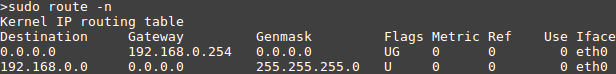
\includegraphics[height=1.3cm]{./imgs/routing-table.png}
          \caption{Routing table}
          \label{fig:routing_table}
        \end{figure}
  \end{frame}

  \begin{frame}
    \frametitle{Routing Principles}
    \begin{figure}[t]
      \centering
      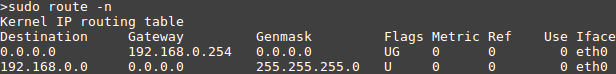
\includegraphics[height=1.3cm]{./imgs/routing-table.png}
      \caption{Routing table}
      \label{fig:routing_table}
    \end{figure}
    \begin{block}{0.0.0.0 ?}
      \begin{itemize}
        \item Default destination
        \item Default (sub)network(s)
        \item Default route
        \item Default gateway
      \end{itemize}
    \end{block}
  \end{frame}

  \begin{frame}
    \frametitle{Routing Principles}
    \begin{block}{Example}
      what would the routing table of this router look like?
    \end{block}
  \end{frame}

  \begin{frame}
    \frametitle{Routing Principles}
    \begin{block}{Static or dynamic ?}
      We will see this later
    \end{block}
  \end{frame}

  \begin{frame}
    \frametitle{CIDR}
    Combine 2+ networks' into one bigger to ease routing.

    \begin{block}{Classless Inter-domain Routing?}
      \begin{itemize}
        \item Can a routing table having both (192.168.0.0/24, E0), (192.168.1.0/24, E0), (10.0.0.0/8, S0) be shorten?
        \item Can a routing table having both (192.168.0.0/24, E0), (192.168.1.0/24, E0), (192.168.8.0/24, E0), (10.0.0.0/8, S0) be shorten?
        \item Can a routing table having both (192.168.0.0/24, E0), (192.168.4.0/24, E0), (192.168.1.0/24, E1), (10.0.0.0/8, S0) be shorten?
      \end{itemize}
    \end{block}
  \end{frame}

  \begin{frame}
    \frametitle{Routing Protocol}
    \begin{itemize}
      \item RIP: Routing Information Protocol
      \item OSPF: Open Shortest Path First
      \item EIGRP: Enhanced Interior Gateway Routing Protocol
    \end{itemize}
  \end{frame}

  \begin{frame}
    \frametitle{Routing Protocol}
      \begin{block}{RIP v1}
        \begin{itemize}
          \item Classful routing
          \item Periodic updates (30 sec) ..
          \item ..by broadcasting (!)
          \item Metric is hop-count (max = 15, infinite = 16)
          \item Timer (180 sec) to tag route as invalid (metric = 16)
          \item no subnet, no VLSM, no CIDR, no router authentication
        \end{itemize}
      \end{block}
  \end{frame}
  \begin{frame}
    \frametitle{Routing Protocol}
      \begin{block}{RIP v2}
        \begin{itemize}
          \item Classless routing
          \item Multicast (224.0.0.9)
          \item VLSM support
          \item Route summarization
          \item "Authentication" (MD5)
        \end{itemize}
      \end{block}

      \begin{center} RIPng is the next RIP version for support of IPv6 \end{center}
  \end{frame}
  \begin{frame}
    \frametitle{Routing Protocol}
      \begin{enumerate}
        \item Router coming online broadcasts Request message
        \item RIP Routers send \textbf{broadcasts} Response messages with their routing table
        \item When Update timers (from other routers) expire, its routing table\footnote{not always the whole table} is sent again
        \item When Invalid timer expires, the metric of the route is set to 16 (unreachable)
        \item When Flush timer expires, the 16-metric routes are removed from the routing table
        \item When a new router (or new metric) is sent, a Hold-down timer is started to stabilize the network.
      \end{enumerate}
  \end{frame}

  \begin{frame}
    \frametitle{Routing Protocol}
    \begin{center}OSPF \end{center}
      \begin{itemize}
        \item Classless
        \item IPv4 and IPv6
        \item VSLM
        \item CIDR
        \item Build a topology of the network
        \item Dijkstra
        \item Metric = f(hop-count, bandwidth, link reliability)
        \item Subdivided into area (a 32-bit number)
        \item Multicast
        \item Authentication support (update only from trusted routers)
      \end{itemize}
  \end{frame}

  \begin{frame}
    \frametitle{Routing Protocol}
    \begin{center}EIGRP \end{center}
      \begin{itemize}
        \item Enhanced IGRP (to support classless routing)
        \item IPv4 and IPv6
        \item VSLM
        \item CIDR
        \item Build a topology of the network
        \item Dijkstra
        \item Metric = f(bandwidth, load, delay, reliability)
        \item Authentication support
      \end{itemize}
  \end{frame}

%% IPv6
  \begin{frame}
    \frametitle{IPv6 - Aims}
    \begin{itemize}
      \item Support billions of hosts (even with inefficient IP addressing)
      \item Reduce routing table size
      \item Simplified protocol to allow routers to process packets faster
      \item Better security
      \item Better real-time QoS
      \item Better multicast diffusion (scope)
      \item Able to move without changing IP address
      \item Give the protocol the ability to evolve
      \item Give the protocol the ability to coexist with newer version
    \end{itemize}
  \end{frame}

  \begin{frame}
    \frametitle{IPv4 vs IPv6}
    \begin{itemize}
      \item not compatible
      \item IPv4 address: 4 octets, IPv6: 16 octets (2$^{128}$ = 3x10$^{138}$)
      \item Packet Header, IPv6: 7 fields, IPv4:13 (faster to process)
      \item IP options: some required options are now optional (faster to process)
      \item Notation:
        \begin{itemize}
          \item 8000:0000:0000:0000:0123:4567:89AB:CDEF
          \item 8000::0123:4567:89AB:CDEF
          \item ::192.168.2.3
        \end{itemize}
      \item Unicast address format:
      \begin{figure}
        \centering
        \begin{tabular}{l|c|c|c}
          bits & 48 (or more) & 16 (or fewer) & 64 \\ \hline
          field & routing prefix & subnet id & interface identifier \\
        \end{tabular}
        \caption{Unicast IPv6 address format}
        \label{fig:uni-ipv6-address}
      \end{figure}
    \end{itemize}
  \end{frame}


  \begin{frame}
    \frametitle{IPv4 vs IPv6}
    \begin{figure}[t]
      \centering
      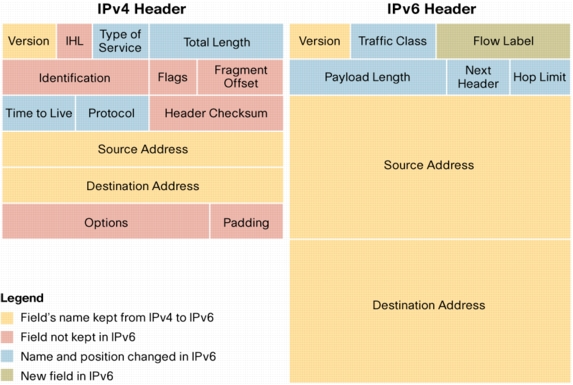
\includegraphics[height=5cm]{./imgs/ipv4-6_header.jpg}
      \caption{IPv4 and IPv6 headers (www.cisco.com)}
      \label{fig:ipv4-ipv6_header}
    \end{figure}
  \end{frame}

  \begin{frame}
    \frametitle{IPv6 - Header}
    \begin{itemize}
      \item \textbf{Version (4 bits):} 0b0110
      \item \textbf{Traffic class (8 bits):} 6-MSB for differentiated services\footnote{multimedia or http}, 2-LSB for ECN\footnote{Explicit Congestion Notification (RFC 3168)}
      \item \textbf{Flow label (20 bits):} routers are supposed to use the same path for the same flow (thus, destination do not need to re-order packets)
      \item \textbf{Payload length (16 bits):} packet length minus its header length
  \end{itemize}
  \end{frame}
    \begin{frame}
      \frametitle{IPv6 - Header}
      \begin{itemize}
          \item \textbf{Next header (8 bits):} specifies the transport layer protocol, also indicates (if any) extension header that follows.
          \item \textbf{Hop limit (8 bits):} Hop count (discussion was to use a duration instead, but router implementations would be much more complex)
    \end{itemize}
    \begin{block}{Optional IPv6 headers offer the possibility to}
        \begin{itemize}
            \item specify the route of the datagram
            \item include authentication data
            \item include fragmentation parameters
            \item and so on...
        \end{itemize}
    \end{block}
  \end{frame}
    \begin{frame}
      \frametitle{IPv6 - Anecdotes}
      \begin{itemize}
        \item IPv6 address length could have been 8 bytes, or 20 bytes, or even variable
        \item Hop count max value (255) is considered, by some, not enough
        \item Removing IPv4 checksum is \emph{as safe as removing brakes from a car}
        \item Different national laws on encryption disallow a real secure transport layer
    \end{itemize}
    \end{frame}

  \begin{frame}
    \frametitle{IPv6 - Adoption}
    \begin{figure}[t]
      \centering
      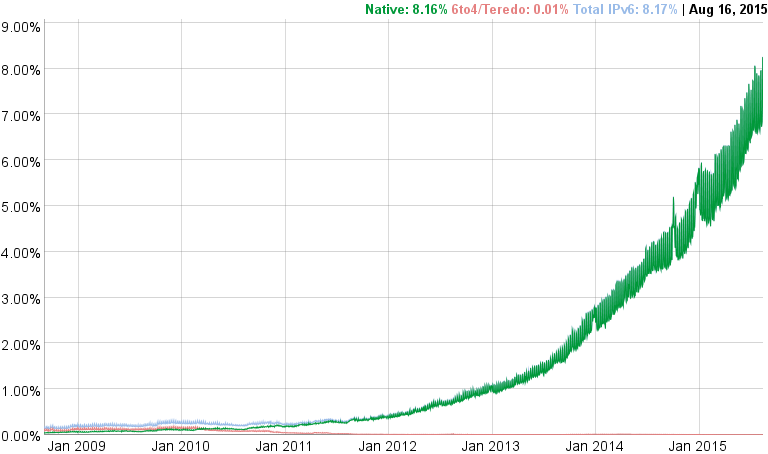
\includegraphics[height=4cm]{./imgs/2015-08-18-IPv6-adoption.png}
      \caption{IPv6 adoption (among Google users)\footnote{https://www.google.com/intl/en/ipv6/statistics.html}}
      \label{fig:ipv6-adoption}
    \end{figure}
    \begin{itemize}
        \item \textbf{2014} Belgium: 28\%, USA and Germany: 11\%
        \item \textbf{2015} Belgium: 36\%, USA: 21\% and Germany: 18\%
    \end{itemize}
  \end{frame}
